%%%%%%%%%%%%%%%%%%%%%%%%%%%%%%%%%%%%%%%%%%%%%%%%%%%%%%%%%%%%%%%%%%%%%%
% writeLaTeX Example: Academic Paper Template
%
% 
% Feel free to distribute this example, but please keep the referral
% to writelatex.com
% 
%%%%%%%%%%%%%%%%%%%%%%%%%%%%%%%%%%%%%%%%%%%%%%%%%%%%%%%%%%%%%%%%%%%%%%
% How to use writeLaTeX: 
%
% You edit the source code here on the left, and the preview on the
% right shows you the result within a few seconds.
%
% Bookmark this page and share the URL with your co-authors. They can
% edit at the same time!
%
% You can upload figures, bibliographies, custom classes and
% styles using the files menu.
%
% If you're new to LaTeX, the wikibook is a great place to start:
% http://en.wikibooks.org/wiki/LaTeX
%
%%%%%%%%%%%%%%%%%%%%%%%%%%%%%%%%%%%%%%%%%%%%%%%%%%%%%%%%%%%%%%%%%%%%%%
\documentclass[twocolumn,showpacs,%
  nofootinbib,aps,superscriptaddress,%
  eqsecnum,prd,notitlepage,showkeys,10pt]{revtex4-1}

\usepackage{amssymb}
\usepackage{amsmath}
\usepackage{graphicx}
\usepackage{dcolumn}
\usepackage{hyperref}
\usepackage{listings}
\usepackage[style=numeric]{biblatex}
\addbibresource{references.bib}

\begin{document}

\title{What is the behavior of Spectre, a speculative prediction exploit, on the various branch predictors available in the computer architecture simulator gem5?}
\author{Kunal Pai}
\affiliation{University of California, Davis}
\author{Yuyi Li}
\affiliation{University of California, Davis}
\author{Frank Gomez}
\affiliation{University of California, Davis}

\begin{abstract}
This project presents a comprehensive investigation into Spectre attacks on x86-based processors, focusing initially on both in-order and out-of-order processors and their susceptibility to speculative execution vulnerabilities. The study employs gem5 v23.0 and Spectre V1, which was compiled on an Ubuntu 16.04 LTS Docker shell with \verb|gcc 4.8.5|. Initial observations highlight the inherent resistance of in-order processors, leading to a focus on only out-of-order processors. Methodological refinements were also built upon the base experiment of running Spectre. These refinements included incorporating extended training periods and exploring the impact of branch predictor state space on Spectre susceptibility. Results confirmed negative correlations between the effectiveness of Spectre and the presence of statistical correctors, loop predictors, a smaller state space, and a less number of training iterations of the branch predictor. The introduction of an extended training period revealed the inherent property of every branch predictor in an out-of-order processor to be vulnerable to Spectre. Therefore, our results help to design the characteristics of a Spectre-resistant branch predictor, proposing features such as statistical correctors, loop predictors, a larger state space, and the use of perceptions. These features aim to prolong the training period and mitigate biased branches, thus reducing the leakage of sensitive information. In conclusion, our findings contribute valuable insights into processor vulnerabilities, offering practical considerations for enhancing Spectre resistance. The presented methodology and results lay the groundwork for future research in developing secure branch predictors and mitigating the impact of speculative execution attacks on modern processors.

Note: the artifacts for our project can be found \href{https://github.com/kunpai/spectre-gem5-v23.0}{here}.
\end{abstract}

\maketitle

\section{Introduction}

In the ever-evolving landscape of computer security, vulnerabilities stemming from the exploitation of hardware components pose significant challenges to maintaining the integrity of sensitive data. One such class of security vulnerabilities, known as Spectre attacks, exploits speculative execution mechanisms in modern processors to gain unauthorized access to confidential information.

Speculative execution, a performance optimization technique employed by contemporary processors, allows the execution of instructions that are predicted to be needed in advance. While speculative execution improves system performance, it introduces a potential avenue for attackers to breach security measures by executing instructions that would not occur during normal program execution. The Spectre attack capitalizes on this vulnerability by manipulating the CPU's speculative execution process to gain access to the victim's memory and registers, ultimately disclosing sensitive data.

This project aims to investigate the behavior of Spectre on various branch predictors available within the gem5 computer architecture simulator. The branch predictors in gem5, such as Tournament, TAGE, Local, Loop, and Bimodal, play a crucial role in guiding speculative execution (by predicting the future direction of branches) and, therefore, present an ideal environment to test how their ``smartness" affects Spectre attacks.

We will also provide an overview of the types of Spectre attacks and their underlying principles. Additionally, we will introduce the gem5 simulator and its relevant CPU models and branch predictors. We would like to explore how various factors within these branch predictors affect the efficacy of Spectre. By exploring these aspects, we seek to contribute to the understanding of Spectre attacks and the development of their mitigations, ultimately strengthening the security of digital systems in an era where data protection is of paramount importance.


\section{Background}

\subsection{What are Spectre attacks?}

Spectre attacks are a class of security vulnerabilities that exploit speculative execution to gain access to sensitive data.

Speculative execution is a technique used by modern processors to improve performance. It works by executing instructions that are predicted to be needed, even if they may not be. This can lead to performance improvements, but it can also be exploited by attackers to gain access to sensitive data.

Spectre attacks work by tricking the CPU into speculatively executing instructions that would not occur during correct program execution. These speculative instructions can access the victim's memory and registers, and can perform operations with measurable side effects. The attacker can then measure these side effects to learn about the victim's sensitive data.

\subsection{Types of Spectre Attacks}

There are several different types of Spectre attacks, but they can all be classified into two main categories\cite{kocher2020spectre}:

\begin{itemize}
\item \underline{Exploiting Conditional Branches}: These attacks exploit the CPU's branch predictor to mispredict the direction of a branch, causing the CPU to speculatively execute code that would not have been executed otherwise. This incorrect speculative execution allows an attacker to read secret information stored in the program’s address space.

Kocher, et. al. found the following:\cite{kocher2020spectre}

If we consider the following piece of code:
\begin{verbatim}
if (x < array1_size) {
    y = array2[array1[x] * 4096];
}
\end{verbatim}

Let's assume that the variable \textit{x} contains data controlled by an attacker. The code includes an \textit{if} statement to check if the value of \textit{x} falls within a valid range before accessing \textit{array1}. The purpose of this \textit{if} statement is to ensure that the memory access to \textit{array1} is valid. However, an attacker can bypass this security measure and potentially read confidential data from the process's memory.

To achieve this, the attacker follows a two-phase approach. In the first phase, they intentionally provide valid inputs to the code, which trains the branch predictor to anticipate that the if statement will evaluate to true. Then, in the second phase, during the actual exploit, the attacker provides a value of \textit{x} that falls outside the allowed bounds of \textit{array1}. Instead of waiting for the branch result to be determined, the CPU makes a speculative guess that the bounds check will pass and begins executing instructions that involve accessing \textit{array2} with a calculation dependent on the malicious \textit{x}. This access loads data into the CPU cache at an address related to \textit{array1[x]} based on the attacker's manipulated \textit{x} value, designed to access different cache lines to avoid prefetching.

Once the bounds check is finally determined, the CPU realizes its mistake and corrects its microarchitectural state. However, the changes made to the cache state are not reverted. This allows the attacker to inspect the cache contents and potentially discover the value of a byte that was retrieved during the out-of-bounds read from the victim's memory, which might contain sensitive information.

\item \underline{Exploiting Indirect Branches}: Kocher, et. al. also found a way to exploit speculative prediction in indirect branches to gain access to private information\cite{kocher2020spectre}. In this variant of the Spectre attack, the attacker utilizes a technique inspired by return-oriented programming (ROP) but with a different approach. Instead of exploiting a vulnerability in the victim's code, the attacker selects a gadget from the victim's address space and manipulates the victim into speculatively executing this gadget. This attack doesn't rely on a specific weakness in the victim's code but rather targets the Branch Target Buffer (BTB) to mispredict an indirect branch instruction, leading to the speculative execution of the chosen gadget. Just like in previous attacks, the CPU's nominal state is eventually corrected, but the effects on the cache are not, allowing the gadget to leak sensitive information through a cache side channel. The attacker demonstrates this empirically and emphasizes that careful gadget selection enables the reading of arbitrary memory from the victim.

To mislead the BTB, the attacker first identifies the virtual address of the gadget in the victim's address space and then performs indirect branches to this address. This training process is conducted from the attacker's address space. The content at the gadget's address in the attacker's address space is not crucial; what matters is that the virtual addresses used during training match or alias those in the victim's address space. Even if there is no code mapped to the virtual address of the gadget in the attacker's address space, the attack can still be successful as long as the attacker handles exceptions appropriately.

\item \underline{Other Variants}: Other variants of Spectre use other methodologies like mistraining return instructions, timing variations, and contention on arithmetic units to leak out information.\cite{kocher2020spectre}
\end{itemize}

Thus, these attacks take advantage of the speculative execution to access and leak information from memory or other sensitive locations that should not be accessible under normal program execution.

\subsection{Spectre code}

We will be using the following code for the Spectre attack\cite{SPECTREPRog}. Our compiler is \texttt{gcc 4.8.5} on Ubuntu 16.04 LTS. As outlined by Lowe-Power\cite{jasonspectre}, a lower compiler version makes a run of Spectre on gem5 much faster. Since we could not replicate the Ubuntu version on which the original version of Spectre was compiled (because it went out of support), we used Ubuntu 16.04, which has long-term support.

This version of the code also, by default, tries to train the branch predictor to predict in one direction 1000 times.

The code works in the following way:

\subsubsection{Victim Code}
The victim code contains a function called \texttt{victim\_function}, which serves as the target for the Spectre attack. It manipulates arrays and aims to leak sensitive data from memory:

\begin{itemize}
  \item \texttt{array1\_size} is set to 16, and \texttt{array1} is an array of 16 bytes.
  \item \texttt{array2} is a larger array used for cache-based timing attacks.
  \item \texttt{secret} is a string containing the sensitive data that the attacker attempts to reveal.
  \item The \texttt{victim\_function} takes an index \texttt{x} as input, and if \texttt{x} is less than \texttt{array1\_size}, it performs a bitwise AND between the current value of \texttt{temp} and the element of \texttt{array2} indexed by the product of \texttt{array1[x]} and 512, and the result is stored back in the temp variable. This operation is designed to leak information.
\end{itemize}

\subsubsection{Analysis Code}
The analysis code is responsible for exploiting the victim function and deducing the value of \texttt{secret}. It employs timing-based attacks to determine whether a specific element of \texttt{array2} was cached, which is dependent on the value of \texttt{x}:

\begin{itemize}
  \item It includes a function called \texttt{readMemoryByte} that repetitively calls the \texttt{victim\_function} with varying \texttt{x} values and observes the time required for memory accesses. Based on the timing information, it infers which elements of \texttt{array2} were loaded into the cache, and consequently, it can make an educated guess about the value of \texttt{x} and, by extension, the value of \texttt{secret}.
  
  \item The code incorporates cache line flushing techniques (using the \texttt{clflush} instruction) to control cache behavior and measure access times. It employs different techniques depending on the availability of instructions and features on the target platform.
\end{itemize}

The main function has a training period of 1000 iterations, and its goal is to train the branch predictor to predict in a certain direction, before calling the victim function and having that direction predicted for the victim function as well.

Therefore, this code employs the first variant of Spectre.

\subsection{What is gem5?}

gem5 is an open-source community-supported computer architecture simulator. Its ecosystem consists of a simulator core and parametrized models for a wide number of components from out-of-order processors, to DRAM, to network devices. The gem5 project consists of the gem5 simulator, documentation, and common resources that enable computer architecture research. \cite{lowepower2020gem5}


Although gem5 boasts a wide range of CPU models, the models of interest for this project are:

\begin{itemize}
    \item \underline{MinorCPU}: MinorCPU is an in-order processor model that offers a fixed pipeline structure but allows for the configuration of its data structures and execution behavior. It encompasses essential pipeline stages like Fetch, Decode, and Execute, making it a valuable tool for studying architectural aspects.\cite{butko2015design}
    \item \underline{O3CPU}: In contrast to MinorCPU, O3CPU is an out-of-order model that features a more complex pipeline with stages including Fetch, Decode, Rename, Issue/Execute/Writeback, and Commit. This model is well-suited for in-depth analysis of speculative execution and its interactions with different branch predictors.\cite{butko2015design}
\end{itemize}

By utilizing these CPU models within gem5, we gain the capacity to explore and assess various architectural scenarios, making a more holistic examination of Spectre attacks and the impact of branch predictors on them.

\subsection{Branch Predictors in gem5}

Looking at the reference code of gem5's Branch Predictors, we can say that gem5 has the following Branch Predictors\cite{Branch}:

\begin{itemize}
    \item \underline{Tournament Branch Predictor}: The tournament predictor as described was originally designed to use one of each category of branch predictors: local and global. The history of each branch is both independent (local) and on a global level.\cite{mcfarling1993combining}
    \item \underline{TAGE Branch Predictor}: This branch predictor relies on a default tagless predictor backed with a plurality of tagged predictor components, indexed using different history lengths. These history lengths form a geometric series. The prediction is provided either by a tag match on a tagged predictor component or by the default predictor. In case of multiple hits, the prediction is provided by the tag-matching table with the longest history.\cite{seznec2006case}
    \item \underline{Local Branch Predictor}: The local branch predictor considers the history of each branch independently and takes advantage of repetitive patterns. Since the histories of branches are independent, it is referred to as local branch prediction.\cite{mcfarling1993combining}
    \item \underline{Bimodal Branch Predictor}: This predictor has a table containing \texttt{n} entries and a 2-bit saturating counter per entry is indexed via the lower-order bits of the PC. The 2 bits are then used as a simple state machine. At each update, the 2-bit counter will be incremented or decremented according to the true result of the branch.\cite{peress2008historical}
    \item \underline{Multiperspective Perceptron Predictor}: This predictor is a hashed perceptron predictor that uses both hashed global path and pattern histories. It also uses a variety of other kinds of features, like an inner-most loop iteration counter and a "modulo-based history",  based on various organizations of branch histories. To access the prediction tables, a feature's hash value is calculated by incorporating recent historical data and hashing it alongside the branch's address to be predicted. This hash value is then adjusted modulo the size of the prediction table. The weight associated with this particular index in the table is retrieved, and all these weights for various features are combined and subjected to a threshold to determine whether the prediction is for the branch to be taken or not.\cite{jimenez2016multiperspective}
\end{itemize}

We will run the Spectre binary on each of these branch predictors in gem5. We plan on having separate configurations for each branch predictor.

\begin{table*}
\centering
\caption{List of Configurations}
\small
\begin{tabular}{p{0.45\linewidth}p{0.45\linewidth}}
% \begin{tabular}{|l|l|}
\hline
X86O3CPU & X86MinorCPU \\
\hline
Tournament BP & Tournament BP \\
BiMode BP & BiMode BP \\
TAGE BP & TAGE BP \\
Multiperspective Perceptron BP (8 kB History size) & Multiperspective Perceptron BP (8 kB History size) \\
Multiperspective Perceptron BP (64 kB History size) & Multiperspective Perceptron BP (64 kB History size) \\
Local BP & Local BP \\
LTAGE (with a loop predictor) & LTAGE (with a loop predictor) \\
TAGE\_SC\_L BP (8 kB History size, with loop predictor and statistical corrector) & TAGE\_SC\_L BP (8 kB History size, with loop predictor and statistical corrector) \\
TAGE\_SC\_L BP (64 kB History size, with loop predictor and statistical corrector) & TAGE\_SC\_L BP (64 kB History size, with loop predictor and statistical corrector) \\
Multiperspective Perceptron TAGE BP (8 kB History size) & Multiperspective Perceptron TAGE BP (8 kB History size) \\
Multiperspective Perceptron TAGE BP (64 kB History size) & Multiperspective Perceptron TAGE BP (64 kB History size) \\
\hline
\end{tabular}
\end{table*}

\subsection{Additional Branch Predictor Components}
Certain components are added onto a base branch predictor in gem5. These components are:

\begin{itemize}
    \item \underline{Loop Predictor}: This predictor involves the use of explicit loop detection for improving the prediction accuracy of loop branches and post-loop branches. Loop detection is implemented by storing information about dynamic instruction sequences that are terminated at backward branches. Additional logic checks for repeating instruction sequences are also implemented. This helps to detect loops.\cite{joseph2000improving}
    \item \underline{Statistical Corrector Predictor}: A downside with branch predictors is that sometimes they fail at predicting statistically biased branches e.g. branches that have only a small bias towards a direction, but are not strongly correlated with the global history path. The Statistical Corrector predictor to better predict this class of statistically biased branches. The predictor aims at detecting the unlikely predictions and to revert them.\cite{seznec2016tage}
\end{itemize}

These additional features are added onto the TAGE predictor in gem5, making the LTAGE (loop predictor) and the TAGE\_SC\_L (both loop predictor and statistical corrector predictor) predictors. They are also added to the Multiperspective Perceptron TAGE BP by default. 

\section{Methodology}

\subsection{Configurations}

The baseline models used will be an x86-based in-order processor and an out-of-order processor.

We will pair each processor up with one of the aforementioned branch predictors and measure some stats from its run that would help us determine how effective Spectre was on it.

Overall, Table I. provides the configurations in more detail:

\subsubsection{Statistics of Interest}

Spectre has already been reproduced in gem5 on the ARM microarchiteture\cite{10.1145/3447852.3458715}, and using the syscall emulation mode in the x86 ISA\cite{jasonspectre}. As part of their methodology, Ayoub and Maurice found that some of the best stats to measure from gem5 that show proof of a more effective Spectre attack are:

\begin{itemize}
  \item \underline{Seconds}: The lower the seconds, the faster a Spectre attack took.
  \item \underline{Number of Mispredicted Branches}: Mispredicted branches are indicative of the smartness of the branch predictor. Lower mispredicts imply that a branch predictor can gauge the pattern across the program more efficiently, making it quicker to train.
\end{itemize}

We will measure these stats as a metric for a run of the Spectre attack\cite{SPECTREPRog} with different branch predictors on the x86 ISA, with the method laid out by Lowe-Power in his blog post\cite{jasonspectre}. We will also measure the percentage of the secret string that was revealed through the output of the Spectre program.

\subsubsection{A Successful Run}
\begin{figure}
    \centering
    \includegraphics[width=\linewidth]{spectreterminal.png}
    \caption{Terminal output of a successful Spectre attack in gem5.}
\end{figure}

To know if a run of Spectre was successful, we will look at the terminal output for leaked information, which is part of the Spectre program we are using. On gem5, a successful run looks like FIGURE 1.



\section{Results}

\subsection{MinorCPU}

The MinorCPU does not show a successful Spectre attack for any branch predictor. The expected secret string is ``The Magic Words are Squeamish Ossifrage.", but any output of the attack when run with a branch predictor on the MinorCPU looks something like the following:

\begin{verbatim}
Reading at malicious_x = 0xffffffffffdd6d48 
... Success: 0xFF='?' score=0
...
\end{verbatim}

While the output says that reading the secret string is a success, it is not, since the character read is from address \texttt{0xFF} and does not contain any character of the secret string either (i.e. 0\% of the secret string revealed).

So, we can say that the Spectre attack \textbf{fails} in an in-order processor in gem5.

\subsection{O3CPU}

For the O3CPU, we noticed a higher success rate in the Spectre attack. All branch predictors were able to reveal at least a part of the secret string, which was of length 40. Table II. provides the exact values for this success rate.

\begin{table}
\centering
\caption{Success Rate of Branch Predictors in the O3CPU with Training Period of 1000 iterations}
\small
\begin{tabular}{p{0.45\linewidth}p{0.45\linewidth}}
% \begin{tabular}{|l|l|}
\hline
Branch Predictor & \% of Secret String Revealed \\
\hline
TAGE BP & 100\% \\
Tournament BP & 100\% \\
Local BP & 100\% \\
BiMode BP & 100\% \\
LTAGE BP & 100\% \\
TAGE\_SC\_L BP (8 kB) & 72.50\% \\
TAGE\_SC\_L BP (64 kB) & 45\% \\
Multiperspective Perceptron BP (8 kB) & 100\% \\
Multiperspective Perceptron BP (64 kB) & 42.50\% \\
Multiperspective Perceptron TAGE BP (8 kB) & 55\% \\
Multiperspective Perceptron TAGE BP (64 kB) & 57.50\% \\
\hline
\end{tabular}
\end{table}
`

\section{Discussion}

\subsection{Impact of Dataflow}
From our results, we can discern that Spectre does not work in an in-order processor in gem5.

In an in-order processor, instructions are executed sequentially in the order they appear in the program. This means that instructions are processed one by one without reordering or speculative execution. Spectre attacks, on the other hand, rely on the processor's speculative predictions, which rely heavily on branch prediction. The predicted branch outcome executes instructions along that path before the actual outcome is confirmed.

Therefore, given no branch predictor could result in a successful Spectre attack, we can say in-order processors are inherently less susceptible to Spectre attacks than out-of-order processors.

\subsection{Impact of Additional Components}
Through our investigations, we find that adding a loop predictor or a statistical corrector makes a branch predictor more resistant to a Spectre attack, and both make the branch predictor even more resistant.

For example, the TAGE branch predictor was the most susceptible to the Spectre attack. From the results, we noticed that adding a loop predictor (LTAGE BP) slowed down the Spectre attack tremendously. However, the secret string was still revealed. But, adding a statistical corrector to the LTAGE branch predictor further slows down the Spectre attack. On top of slowing it down, in both variants of the TAGE\_SC\_L BP, the secret string is not fully revealed.

Even in the Multiperspective Perceptron, the variants that add a loop predictor and a statistical corrector (i.e., the Multiperspective Perceptron TAGE BP variants) slow down the time taken for a Spectre attack, and do not reveal the entire secret string.

This is in line with the functions of these two components.

Loop predictors are designed to identify loops in the code and predict the outcomes of branch instructions within those loops more accurately. Spectre attacks often rely on exploiting the speculative execution of branch instructions. By enhancing the prediction of branch instructions within loops, it becomes more difficult for attackers to steer the speculative execution in a way that leaks sensitive data.

Branch predictors are also designed to make predictions based on historical behavior and patterns but, some branches have a bias towards a particular direction, making them challenging to predict accurately. Spectre attacks often target such branches. The statistical corrector is designed to detect when the branch predictor's predictions are statistically biased or unlikely, and it can help revert these unlikely predictions. This correction mechanism can prevent the branch predictor from speculatively executing instructions that could be exploited by a Spectre attack.

Therefore, by adding these two components to the branch predictor, it becomes more robust against attacks that rely on exploiting statistically biased branches, since they take more iterations to be trained to mispredict. This makes it more difficult for an attacker to leverage these branches to leak sensitive information.

\subsection{Impact of ``Smartness" of BP}

Our results indicate that the ``smartness" of the branch predictor, i.e., less training to get more accurate predictions, is a major factor in how susceptible it is to Spectre. The trend observed is that the ``smarter" the branch predictor is, the more susceptible it is to Spectre.

\begin{figure}
    \centering
    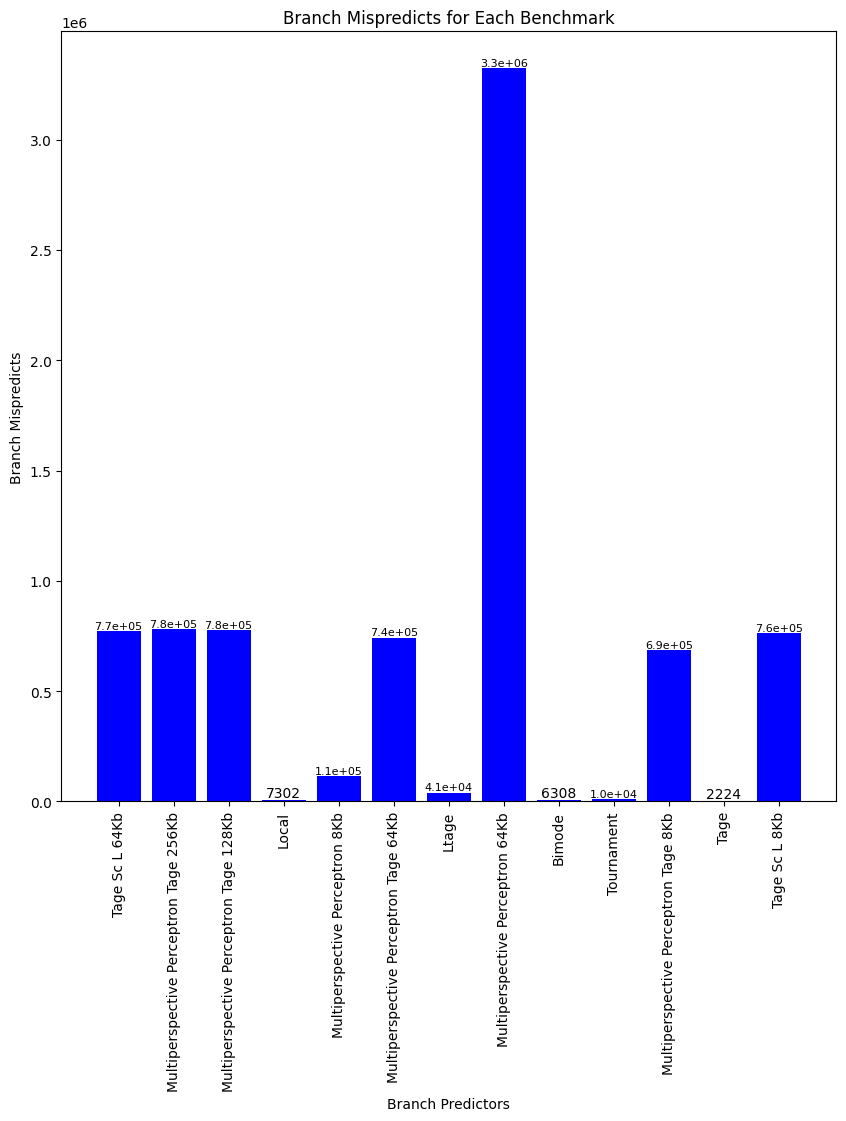
\includegraphics[width=\linewidth]{Branch Mispredicts.png}
    \caption{Branch mispredictions per branch predictor type of a base Spectre attack in gem5.}
\end{figure}

\begin{figure}
    \centering
    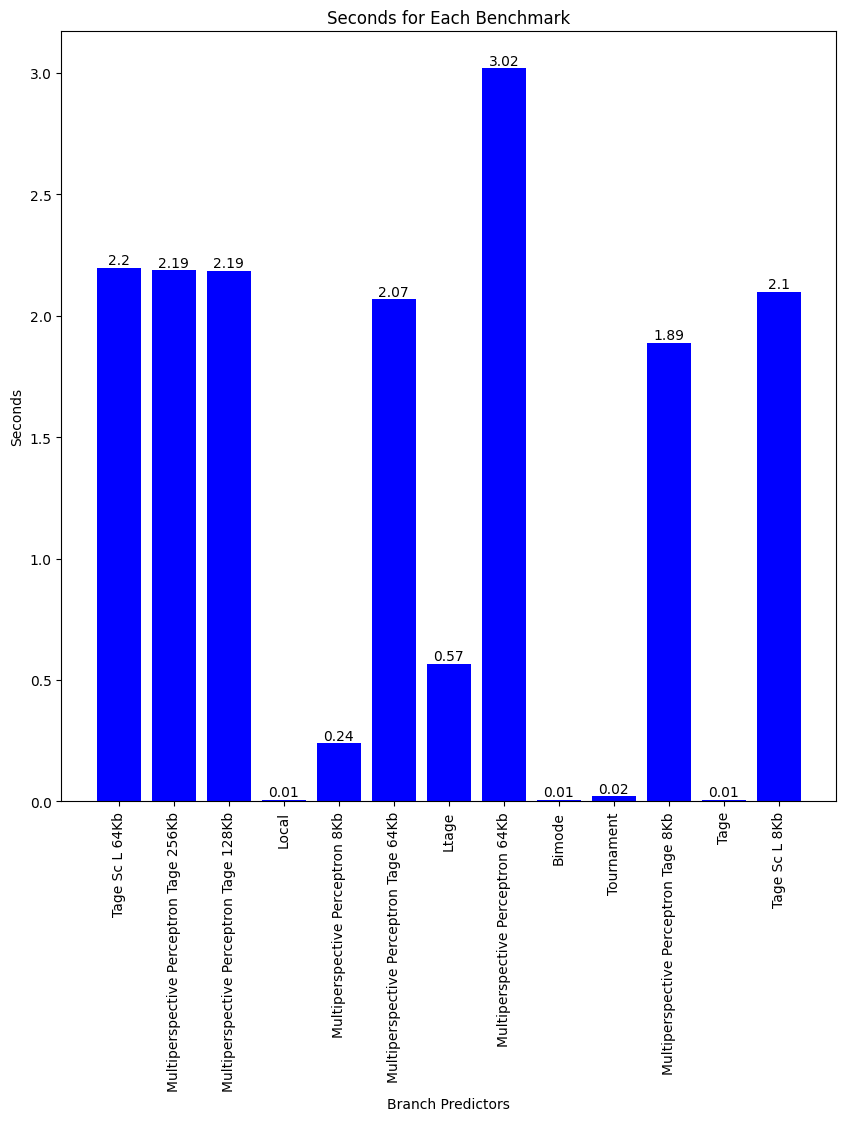
\includegraphics[width=\linewidth]{Seconds.png}
    \caption{Seconds taken to complete a base Spectre attack per branch predictor type in gem5.}
\end{figure}

If we were to look at the total branch mispredictions per branch predictor in gem5 in Fig. 2 and the time it took for the Spectre attack to complete, we can see that the ``smartest" branch predictor, the TAGE, with the least mispredictions, was the most susceptible to Spectre, using time as a metric for efficacy. It only took 0.008 seconds for the entire secret string to be revealed.

Conversely, if we look at the Multiperspective Perceptron 64 kB branch predictor, the Spectre attack took the longest (3.02 seconds) and the branch predictor had the most mispredicts too. Even the secret string was not fully revealed.

It makes sense why TAGE would be more susceptible than the MPP branch predictor. 

TAGE predictors are known for their rapid training and accuracy. They use a combination of several tables to track the history of recent branch outcomes and make predictions. These tables allow TAGE predictors to adapt quickly to the behavior of the program because they can learn from the recent history of branches. TAGE predictors have also implemented parallelism to do this even faster, meaning that they are more likely to understand the trend of the branch the quickest. Thus, they can be easily exploited by attackers.\cite{seznec2006case}

Multiperspective Perceptron, on the other hand, is a more complex branch predictor. It uses perceptrons to capture various features and perspectives of the branch history. Training a structure such as the Multiperspective Perceptron, involves more extensive calculations and adjustments of weights. This process is more time-consuming compared to traditional table-based predictors like TAGE. Additionally, the Multiperspective Perceptron requires more training data and iterations to converge to an accurate prediction model, which contributes to a longer training time.\cite{jimenez2001dynamic}

As a way to counter the downside of a huge training time, the MPP TAGE branch predictor was introduced, and it predicts better, as evident from Fig. 2. But the tradeoff is that it is more vulnerable to Spectre, as evident from Fig. 3.

We can also explain the trends in the other branch predictors using their structure and prediction mechanisms.

Local branch predictors make predictions based on the local history of a single branch instruction, typically using a small table for each instruction. The training of local predictors involves updating these local history tables when the branch outcome is known. Since the tables are small and specific to each branch instruction, training can be done quickly, but not as quickly as TAGE due to lack of parallelism.\cite{mcfarling1993combining}

Bimodal branch predictors use a two-bit saturating counter to make predictions based on the overall behavior of branch instructions. Training the bimodal predictor involves updating this single table when branch outcomes are known, which is a straightforward process and can be done quickly, but again not as quickly as TAGE due to lack of parallelism.\cite{peress2008historical}

Tournament predictors combine multiple branch predictors, such as local and global predictors, to select the most accurate prediction for a given branch instruction. Training a tournament predictor involves training its individual components (e.g., local and global predictors) and adjusting the selection mechanism. While the training process for tournament predictors is more involved than simple local or bimodal predictors, it is typically faster and less complex than training the Multiperspective Perceptron, and still slower than TAGE due to lack of parallelism.\cite{mcfarling1993combining}

It seems like the easier the branch predictor can be trained to predict in a certain direction

\subsection{Impact of BP State Space}

From our observations, we notice that increasing the state space of the branch predictor could help mitigate the Spectre attack.

We already notice this trend with the TAGE\_SC\_L BP and the Multiperspective Perceptron BP, where increasing the size of the branch predictor from 8 kB to 64 kB helps mitigate the Spectre attack by revealing less of the secret string, from 72.50\% to 45\% and from 100\% to 42.50\% respectively.

This observation makes sense. A larger branch predictor can store and manage more information about program control flow, including speculative execution paths. With a larger predictor, the processor can make more accurate predictions about which branches to take, which means it can speculatively execute code more effectively. This makes it more challenging for an attacker to influence the speculative execution to leak sensitive data. Since a larger branch predictor has more "states" to work with, it becomes difficult to train the branch predictor to just pick one direction and then mispredict. Therefore, within the \textbf{limited iterations} of the Spectre code, it is difficult to train a larger state space than a smaller one, which is why larger branch predictors reveal less of the secret string. 

An outlier in this data seems to be the Multiperspective Perceptron TAGE BP, where increasing the size reveals 1 more character of the secret string, but a theory as to why that happens could be the difference in the implementation of the TAGE and the statistical corrector that is used in both variants of the branch predictor.

To confirm our hypotheses, we took the Multiperspective Perceptron TAGE BP with the 64 kB implementation of the loop predictor and the statistical corrector and changed the number of budget bits, effectively changing the size of the BP. We found that increasing the size still mitigates against Spectre, and these findings are summarized in Table III.

\begin{table}
\centering
\caption{Success Rate of Budget Bits of the Multiperspective Perceptron TAGE BP - 64 kB TAGE, LP and SC}
\small
\begin{tabular}{p{0.45\linewidth}p{0.45\linewidth}}
\hline
Number of Budget Bits & \% of Secret String Revealed \\
\hline
67584 & 45\% \\
526336 & 57.50\% \\
1048576 & 50\% \\
2097152 & 45\% \\
4194304 & 47.50\% \\
8388608 & 47.50\% \\
\hline
\end{tabular}
\end{table}

\begin{figure*}
    \centering
    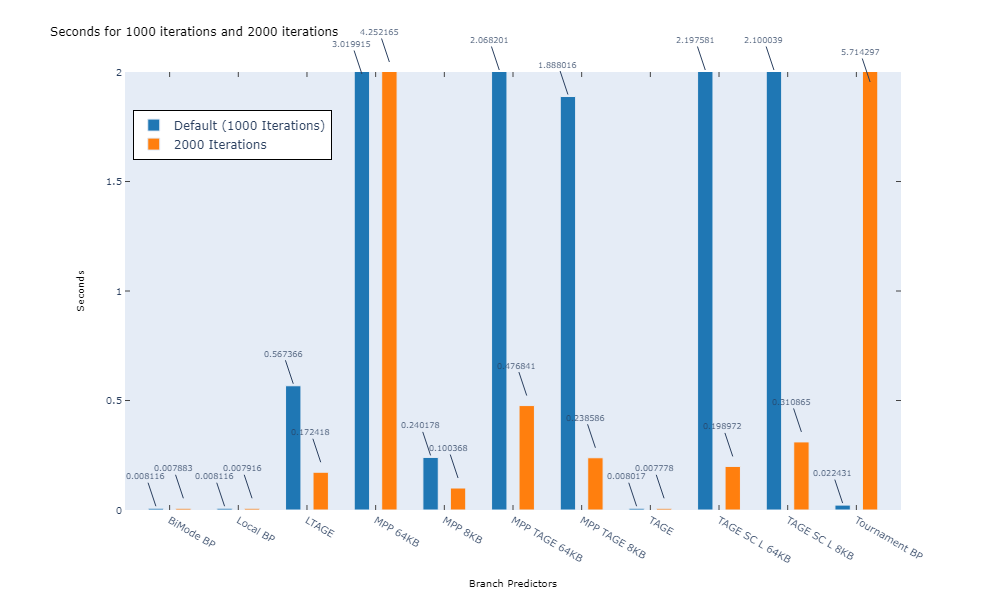
\includegraphics[width=\linewidth]{SecondsAndIterations.png}
    \caption{Seconds taken to complete a base Spectre attack per branch predictor type in gem5.}
\end{figure*}

While increasing the state space does not guarantee mitigation of Spectre, it can still be considered as a potential mitigation strategy, albeit not as strong as other approaches. Expanding the state space potentially increases the difficulty for attackers to manipulate the branch predictor and execute Spectre attacks. However, the effectiveness of this approach is not consistent and requires further research and validation. Ultimately, a combination of mitigation strategies, including increasing the state space alongside other techniques, is likely necessary for comprehensive protection against Spectre.

% Since Spectre is based on training the branch predictor to predict in one direction, this can be performed on any branch predictor, and is a matter of chance.
\subsection{Impact of Training Period of Branch Predictor}

Since Spectre is based on training the branch predictor to predict in a certain direction, we also wanted to see if increasing the training period could reveal more of the secret string. So, we reran the configurations with a version of the Spectre binary that trains the branch predictor for \textit{twice} the number of iterations, i.e., 2000.

gem5's MinorCPU still did not reveal any part of the secret string for any branch predictor. Even with an extended training period, the MinorCPU configuration did not exhibit any susceptibility to Spectre attacks, which strengthens the claim that the nature of the processor itself makes it more resistant to Spectre.

Regarding the O3CPU, we observed an increase in the percentage of characters revealed in the secret string. Our findings are summarized in Table IV.

\begin{table}
\centering
\caption{Success Rate of Branch Predictors in the O3CPU with Training Period of 2000 iterations}
\small
\begin{tabular}{p{0.45\linewidth}p{0.45\linewidth}}
% \begin{tabular}{|l|l|}
\hline
Branch Predictor & \% of Secret String Revealed \\
\hline
TAGE BP & 100\% \\
Tournament BP & 100\% \\
Local BP & 100\% \\
BiMode BP & 100\% \\
LTAGE BP & 100\% \\
TAGE\_SC\_L BP (8 kB) & 100\% \\
TAGE\_SC\_L BP (64 kB) & 100\% \\
Multiperspective Perceptron BP (8 kB) & 100\% \\
Multiperspective Perceptron BP (64 kB) & 85\% \\
Multiperspective Perceptron TAGE BP (8 kB) & 100\% \\
Multiperspective Perceptron TAGE BP (64 kB) & 100\% \\
\hline
\end{tabular}
\end{table}

Remarkably, the O3CPU configuration exhibited an increase in the percentage of characters revealed in the secret string, indicating that a more extended training period positively influenced the success of the Spectre attack. Notably, the success rates were 100\% across various branch predictors.

This finding aligns with the overarching statement that ``\textit{any branch predictor can be trained to predict in a specific direction}".

In cases where the Spectre attack succeeded completely with 1000 iterations, it takes much shorter with 2000 iterations. This is because a longer training period of the branch predictor implies that it is surer of the direction to predict. the extended training may have introduced more consistent or reliable predictions. The additional training data also has reinforced the existing prediction patterns, making the speculative execution more efficient and reducing the time required for the Spectre attack to successfully leak sensitive information.

In cases where the Spectre attack did not succeed completely with 1000 iterations, it also takes much shorter with 2000 iterations, since we are training the branch predictor more effectively. The increased number of iterations enhances the training of the branch predictor, allowing the attacker to more effectively manipulate speculative execution and extract targeted information. This shorter timeframe for success in the extended iteration scenario is attributed to the refined training of the branch predictor.

An outlier in these trends is the Tournament branch predictor, which takes longer with 2000 iterations, even though it reveals the entire secret string in both, and the Multiperspective Perceptron 64kB, which reveals a little bit more of the secret string with 2000 iterations, but still does not reveal it entirely. 

The reason for these outliers is that the tournament predictor has a more complex training mechanism. This branch predictor combines multiple branch predictors, such as local and global predictors, to select the most accurate prediction for a given branch instruction, in a tournament format. So, every iteration takes a fixed amount of time to train the branch predictor. This is why more iterations take longer.

Similarly, for the Multiperspective Perceptron, since every prediction considers a lot of factors, the extended training may introduce more nuanced patterns, making the prediction process more complex and time-consuming. The Multiperspective Perceptron likely requires additional iterations to refine its understanding of the branch behavior and the relationships between the different factors it considers in a prediction. Since reading the data from the cache in an unsuccessful attempt also takes longer than a successful attempt, both these delays add up to make this branch predictor have a longer delay.

Overall, our results imply that every branch predictor can be trained to predict in a certain direction, and is susceptible to a Spectre attack. An attacker, with a sufficiently long number of training iterations, can exploit the branch predictor to reveal secret information.

\section{A Secure Branch Predictor}

With a large enough training period, Spectre would be able to reveal details from memory no matter the branch predictor. The goal of the branch predictor in this case is to extend the time it takes for training and try to mitigate biased branches as much as possible so that fewer details of the memory are leaked out.

Given the above analysis, we tried to ask the question: \textit{What would the characteristics of the most Spectre-resistant branch predictor look like?}

We conclude it would have the following features:
\begin{itemize}
    \item A statistical corrector and a loop predictor to make sure that the branch predictor cannot be trained to predict in one direction very quickly.
    \item A larger state space, meaning that it has a larger history table of branches' results.
    \item Perceptrons to capture various features and perspectives of the branch history. Training a structure like this involves more extensive calculations and adjustments of weights, which is more holistic than a traditional table-based system.
\end{itemize}

\section{Conclusion}
Our investigation into Spectre attacks on x86 processors has shed light on critical insights, revealing the vulnerabilities and potential mitigations within diverse branch predictors. Through our research, we confirmed the effectiveness of statistical correctors and loop predictors in reducing Spectre's impact. Also, we found that rapidly trained branch predictors were found to be more susceptible. This analysis led to the exploration of a Spectre-resistant branch predictor, which we characterize to be one with a statistical corrector, loop predictor, larger state space, and perceptrons. These features advocate for a holistic training approach, serving not only to extend the training period but also to reduce swift, biased directional predictions, thereby mitigating Spectre. With speculative execution attacks like Spectre posing an ongoing threat, our research efforts remain crucial in fortifying processors against these sophisticated threats.



% \subsection{Mathematics}

% \LaTeX{} is great at typesetting mathematics. Let $X_1, X_2, \ldots, X_n$ be a sequence of independent and identically distributed random variables with $\text{E}[X_i] = \mu$ and $\text{Var}[X_i] = \sigma^2 < \infty$, and let
% $$S_n = \frac{X_1 + X_2 + \cdots + X_n}{n}
%       = \frac{1}{n}\sum_{i}^{n} X_i$$
% denote their mean. Then as $n$ approaches infinity, the random variables $\sqrt{n}(S_n - \mu)$ converge in distribution to a normal $\mathcal{N}(0, \sigma^2)$.

% \subsection{Lists}

% You can make lists with automatic numbering \dots

% \begin{enumerate}
% \item Like this,
% \item and like this.
% \end{enumerate}
% \dots or bullet points \dots
% \begin{itemize}
% \item Like this,
% \item and like this.
% \end{itemize}

% \begin{acknowledgments}

% We thank\dots

% \end{acknowledgments}

\printbibliography

\end{document}